\documentclass[UTF8]{ctexart}
\usepackage{graphicx}
\graphicspath{{img/}} 
\title{Homework\ 4}
\author{PB17111623}
\author{PB17111623 范睿}
\date{\today}
\usepackage[a4paper,bottom=3.5cm]{geometry}
\usepackage{algorithm}  
\usepackage{algorithmicx}
\usepackage{amsmath}  
\usepackage{algpseudocode}  %算法的包
\usepackage{amssymb}
\begin{document}
\maketitle
\section{}
\subsection{下面的排序算法中哪些是稳定的:插入排序、归并排序、堆排序、快速排序和计数排序?给出一个能使任何排序算法都稳定的方法。你所给出的方法带来的额外时间和空间开销是多少?}
稳定的排序算法:插入排序、归并排序、基数排序\\
不稳定的排序算法:堆排序、快速排序\\\\
方法:利用一个结构体类型存放每一个数值,结构体中有两个元素,第一个是data,存放数列中的元素,第二个是index,存放每一个元素被读入时的次序。然后按照任何一种算法根据data排序。在排序的过程中,如果遇到两个data相同的元素,则比较index项,将index小的那一项排在前面。\\\\额外的时间开销:每一次交换操作增加了一个值+比较过程增加了一个比较index的分支\\
额外的空间开销:利用了原来两倍的空间来存放data和index
\subsection{假设用 Random-Select 去选择数组 A = (3,2,9,0,7,5,4,8,6,1)的最小元素,给出能够导致Random-Select 最坏情况发生的一个划分序列。}
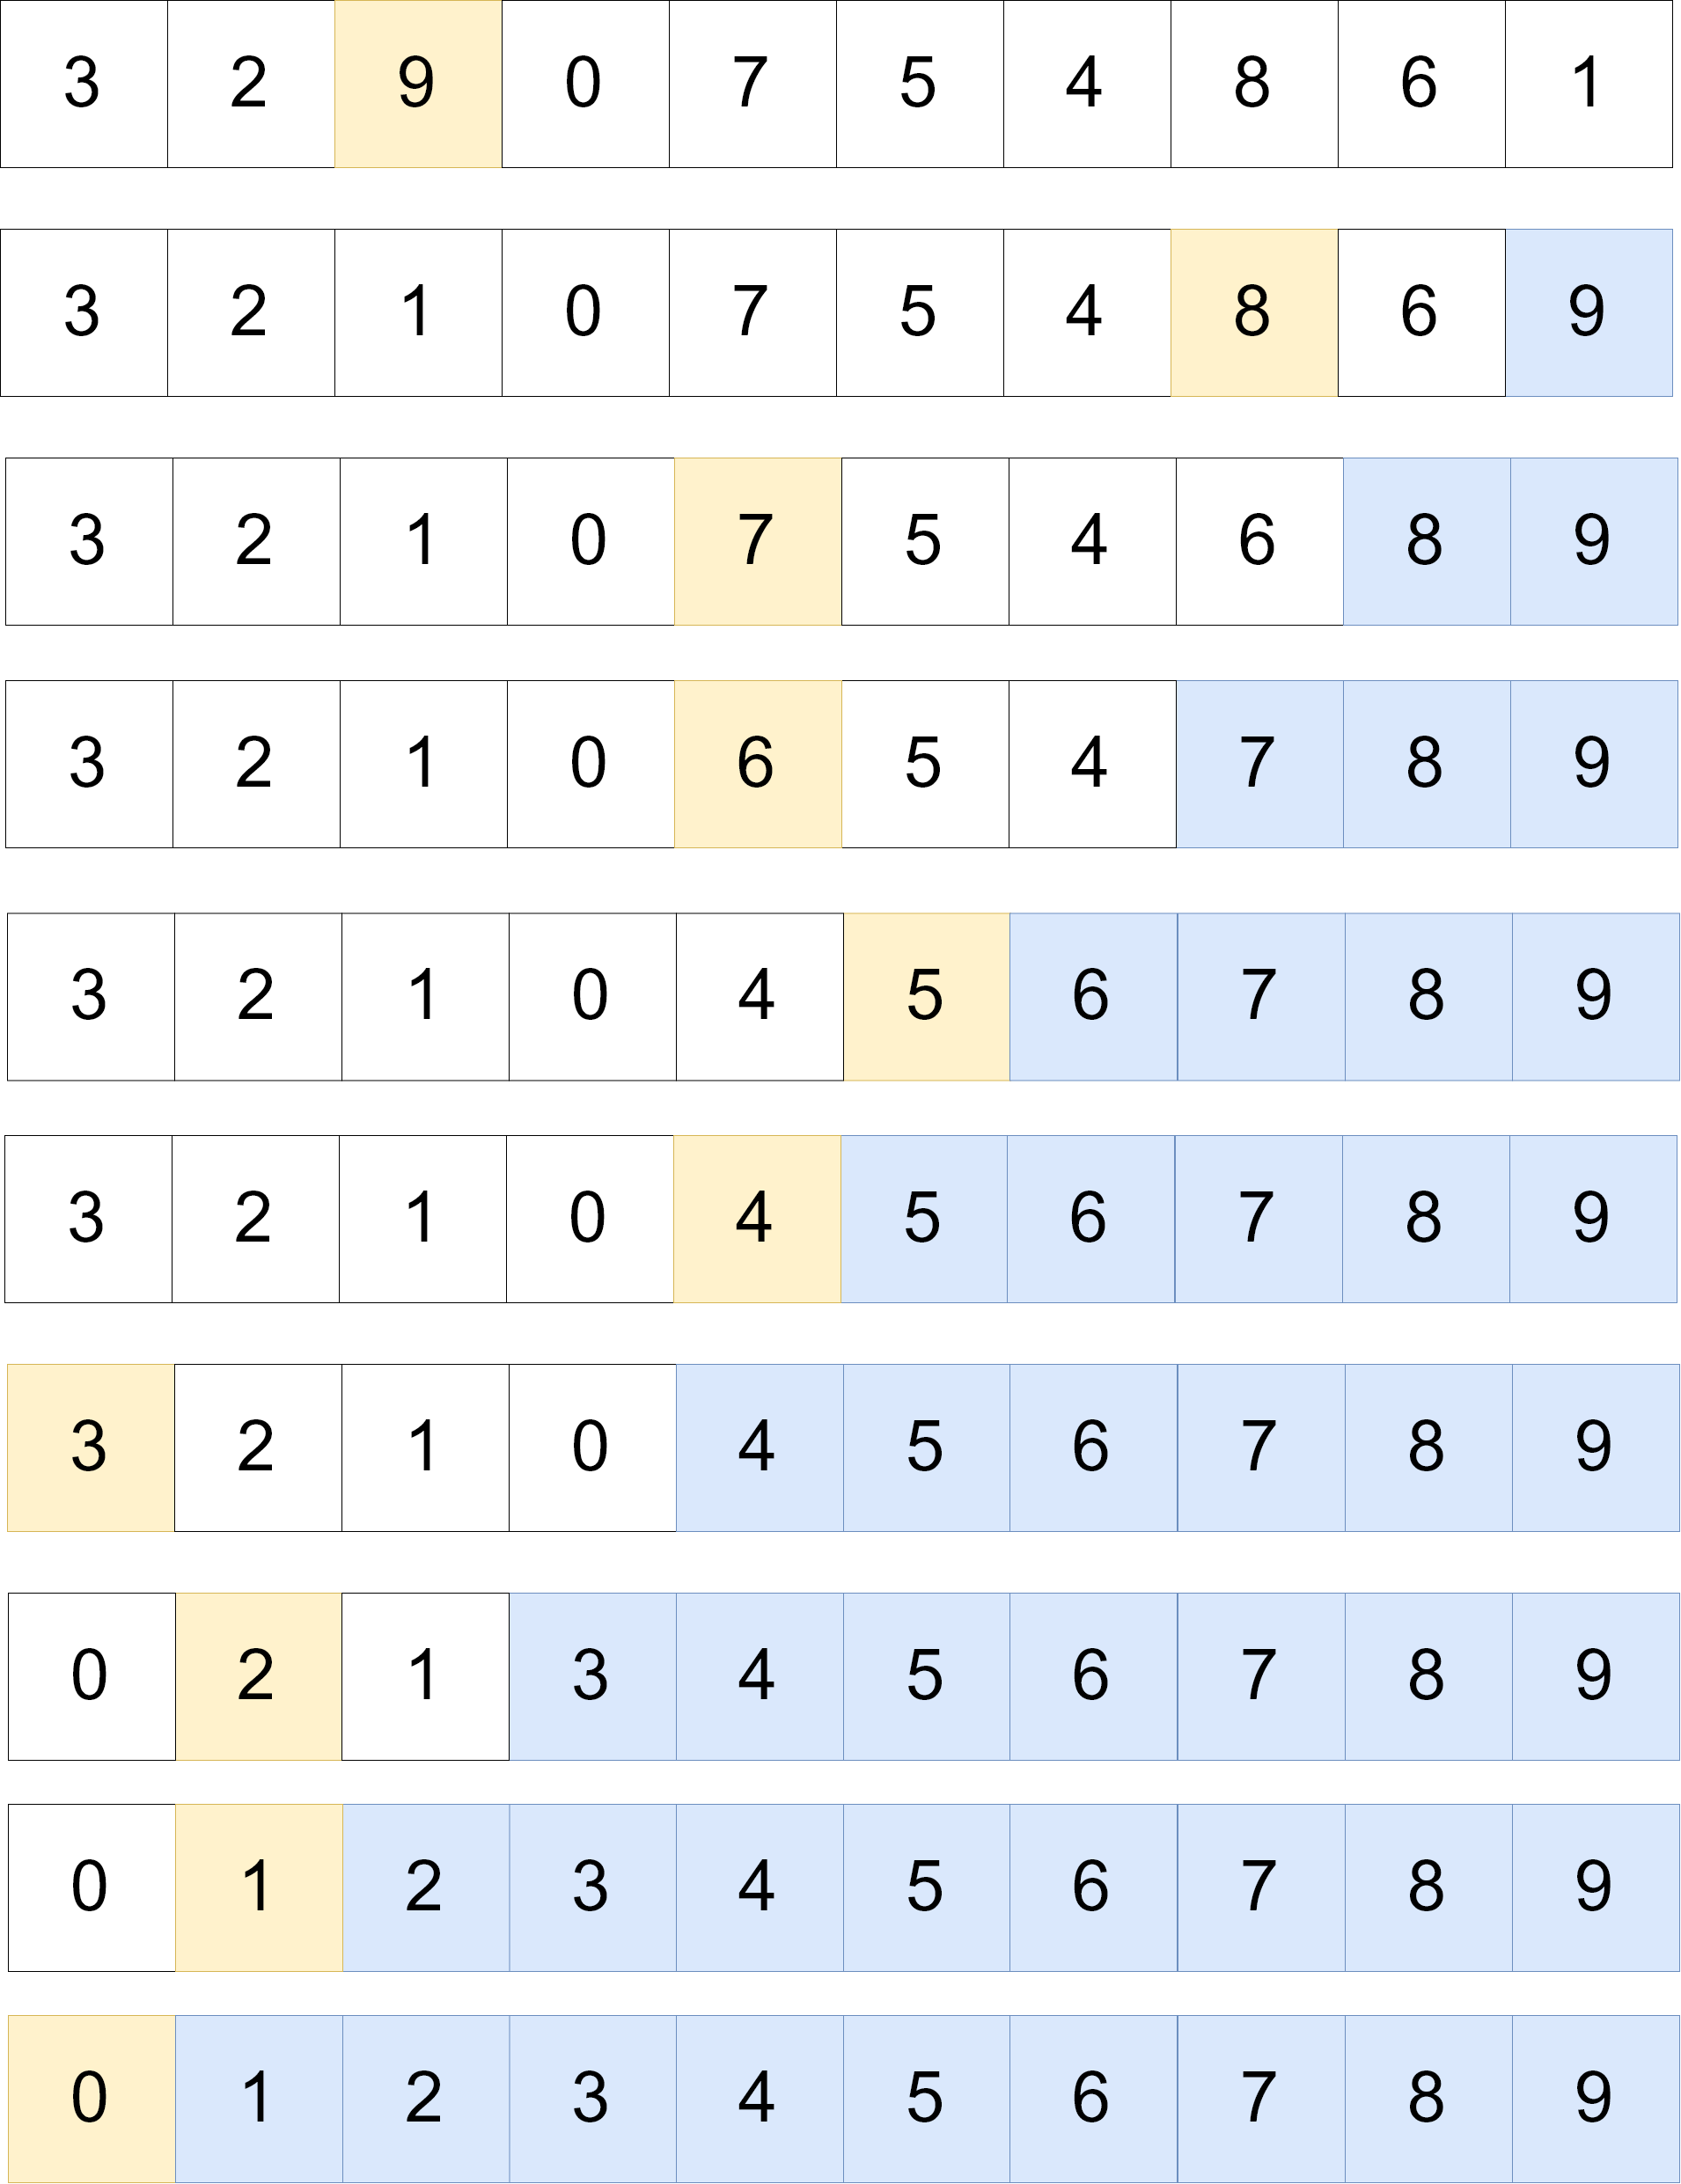
\includegraphics[scale=0.2]{img/partition.png}

\end{document}